
Over the past 100 years, roads have become more and more congested. The number of vehicles on the road in the UK alone has increased by more than 50\% since 1994\cite{AllVehiclesVEH01}, this is thought to be considerably higher in developing countries, and the trend over the past decade is a 1-2\% growth year-on-year. This can be seen in Figure~\ref{fig:vehicles-time}. All the while, road networks in countries such as the UK are not being extended, putting the existing infrastructure under increasing strain.

Human piloted vehicles however, on top of this, do not efficiently utilise the roads available, requiring additional space per vehicle due to factors such as \textit{reaction time}, if we were able to remove these human elements it would be possible to greatly increase the throughput of the same amount of road infrastructure.

We can also consider the impact of autonomous navigation on road fatality rates. Over the past 10 years there have been an average of 1984 deaths per year on UK roads\cite{ReportedRoadCasualties}, with around a further 24,000 people seriously injured. Many of these incidents will have occurred due to human error, error which could be eliminated if the human factor were to be removed from vehicle navigation and routing and replaced with a robust, reliable automated system.


\begin{figure}[ht]
  \centering
  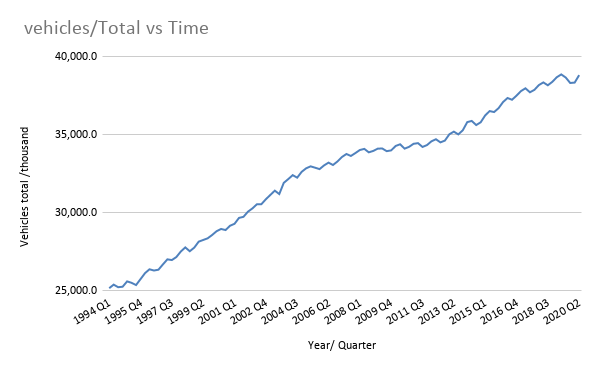
\includegraphics[scale=0.5]{figures/vehicles-time.png}
  \caption{\label{fig:vehicles-time} Total vehicles registered on UK roads over time\cite{AllVehiclesVEH01}}
\end{figure}


\todo[inline]{Lay out different tasks \& steps of the project, identify subgoals}
\section{Goals}

The overarching goal of this project is to optimally route traffic in the setting of a fully-autonomous road system. This however, is an aspirational goal with many sub-requirements to be fulfilled before it can come to fruition.

Formally this top-level goal can be said to be to answer the question in Problem~\ref{prob:Spec}.

\begin{figure}[htpb]
    \centering
    \begin{problem}{prob:Spec}

        \problemtitle{Top-level Goal}
        \probleminput{ 
            \begin{itemize}
                \item A road system $\mathcal{R}$ represented as a graph $\mathcal{R} = (V,E)$


                    Where each edge $e \in E$ is a section of road defined as the space between two vertices $v^1,v^2 \in V$ which is bounded by two functions $b_1(x)$ and $b_2(x)$ and augmented by a set of obstacles $O$ representing infeasible sections of road space
                \item a set of agents, $A = \left\{ a_1,\ldots,a_n \right\}$
                \item a list of vertex pairs representing start and goal points for each agent:

                    $\mathcal{V} = \left\{ (v_1^1,v_1^2),\ldots, (v_n^1, v_n^2) \right\}, v_{i \in [1 \ldots n]}^{j \in [1,2]} \in V$

                where the route for agent $a_i$ is from vertex $v_i^1$ to $v_i^2$
            \end{itemize}
        }
        \problemquestion{ What is the set of optimal routes $\mathcal{V}_{optimal}$, where the $i^{\text{th}}$ element  is defined as a set of linked Bézier curves connecting $v_i^1$ and $v_i^2$ through feasible space?}
        \end{problem}
\end{figure}

We can then split this into more manageable sub-goals. The sub-problem of generating a route through a section of road is defined in Problem~\ref{prob:sub1}. This can be further decomposed into the selfish routing of a single agent through a section of road defined in Problem~\ref{prob:sub2}

\begin{figure}[htpb]
    \centering
    \begin{problem}{prob:sub1}
        \problemtitle{Sub-Goal: Cooperative route planning}
        \probleminput{
            \begin{itemize}
                \item A start point $P_{start}$ and a goal point $P_{goal}$ 
                \item A section of road as defined in Problem~\ref{prob:Spec}
                \item A knowledge of all routes being planned to be executed concurrently.
            \end{itemize}
        }
        \problemquestion{What is the optimal route, in the form of a Bézier curve, between these two points s.t. it does not collide with any other agents or pass through any infeasible regions in the road space?}
    \end{problem}
\end{figure} 

\begin{figure}[htpb]
    \centering
    \begin{problem}{prob:sub2}
        \problemtitle{Sub-Goal: Single agent route planning}
        \probleminput{
            \begin{itemize}
                \item A start point $P_{start}$ and a goal point $P_{goal}$ 
                \item A section of road as defined in Problem~\ref{prob:Spec}
            \end{itemize}
        }
        \problemquestion{What is the optimal route, in the form of a Bézier curve, between these two points s.t. it does not pass through any infeasible regions in the road space?}
    \end{problem}
\end{figure} 

\begin{figure}[htpb]
    \centering
    \begin{problem}{prob:sub3}
        \problemtitle{Sub-Goal: Bézier curve generation}
        \probleminput{
            \begin{itemize}
                \item A start point $P_{start}$ and a goal point $P_{goal}$ 
                \item A section of road as defined in Problem~\ref{prob:Spec}
            \end{itemize}
        }
        \problemquestion{What is the optimal route, in the form of a Bézier curve, between these two points s.t. it does not pass through any infeasible space?}
    \end{problem}
  \end{figure}

\subsection{Requirements}
\label{subsec:requirements}

The goal of this project was not to produce a production-ready system, but instead, to investigate the plausibility of GAs on the real future possibility of completely autonomous road networks. As such I feel it useful to outline the theoretical requirements of a production grade system. To do this formally I will employ Propositional and Temporal logic.

\begin{enumerate}
\item The system should never return a set of routes such that, for any time $t \in T, \forall i \in n, \forall j \in n, j \neq n, I_{i}(t) = I_{j}(t)$. I.e. for any time, no routes should inhabit the same point, meaning there are no collisions in the planned routes.\todo{This is wrong, correct this or remove it outright}
\end{enumerate}

%TC:macro \todo 1

%%% Local Variables:
%%% mode: latex
%%% TeX-master: "report"
%%% End:
